\section{Introduction}
\label{sec:intro}

An agent that plans or learns inside a model of its environment can only use what that model represents.
World models compress observations into a latent state from which future observations, rewards, and episode ends can be predicted. They then train a policy on imagined rollouts of that state rather than on the environment \citep{ha2018worldmodels,hafner2019planet,hafner2020dreamer}.
DreamerV3 \citep{hafner2023dreamerv3,hafner2025dreamerv3nature} made this recipe work across domains with fixed hyperparameters, and world models now range from interactive video simulators \citep{bruce2024genie,hafner2025dreamer4} to theory arguing that general agents must contain one \citep{richens2025general}.
What the latent state of a reconstruction-trained world model represents, however, is decided mostly by a pixel loss.
That loss weighs every pixel equally and is dominated by large, frequent regions of the frame; small task-critical elements can drop out of the reconstruction entirely \citep{burchi2024mudreamer}.
A decision that depends on one small tile, such as crafting next to a workstation, gives the reconstruction loss almost nothing to pay for.
Recent probing work shows that a model can predict well while encoding an incoherent picture of the world \citep{vafa2024evaluating,gonzalezlaiz2026limits}.
This raises a representation question that a return curve cannot answer: \emph{does the agent's learned state contain the fact its rare decision depends on?}

We study this question with \method{}, a recurrent state-space model (RSSM) in the DreamerV3 family with one addition: a \emph{field head}.
The field head reads the latent state and predicts a local symbolic map, with a material class and an object class in each cell around the agent.
The actor reads that map alongside the latent features.
Imagination has no environment state, so in imagination the actor reads the field head's prediction.
In every run reported here, the actor reads the environment's true map on real steps, including evaluation.
We repeat this split throughout because it bounds what the experiments can show.

The field head turns the question into a measurement: \emph{does the latent name the tile the action needs?}
We pair the probe with two training conditions that should matter if the answer is no.
The first is where the action-relevant tile sits relative to the field: inside it while the demonstrator approaches, or outside it.
The second is whether training windows sampled from demonstrations are anchored to end on the rare action, or are ordinary slices that usually miss it.
We run both conditions on Crafter \citep{hafner2022crafter} with a large model and in a small controlled room with a small model, and report the same measurements in both.
\Cref{fig:example} shows the central observation on one benchmark frame.

\begin{figure}[t]
  \centering
  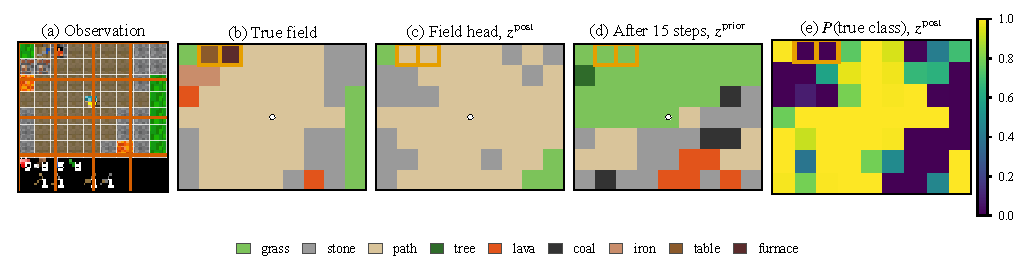
\includegraphics[width=\linewidth]{field_example.pdf}
  \caption{What the latent names on one benchmark frame (beside-resource anchored run, 100k steps). (a)~The $64\times64$ observation with Crafter's 7-pixel tiles (white) and the $16\times16$-pixel cells of the encoder's final feature map (orange): one latent cell spans more than two tiles in each direction. (b)~The true $9\times7$ field; the station tiles are outlined. (c)~The field head's prediction from the posterior latent: terrain is largely right (\ExamplePostAcc\% of cells), but the station is replaced by path, with probability \ExamplePostTable{} on the table tile. (d)~The same field after 15 imagined steps from the prior, the horizon on which the actor is trained: the map has drifted toward grass (\ExamplePriorAcc\% of cells). (e)~Probability of the true class per cell under the posterior. The frame is the probe frame with the most station cells in daylight; \cref{sec:latent} gives statistics over all \FieldCells{} probed cells.}
  \label{fig:example}
\end{figure}

\paragraph{Findings.}
\begin{itemize}
  \item \emph{On Crafter, the latent names terrain and not the station.} Probed on \FieldCells{} cells from eight demonstrator lives, the field head is correct on 72\% of cells, against \FieldBaseline\% for predicting the most common class everywhere. It assigns the true class a mean probability of 0.92 on grass, about 0.52 on stone, and 0.13--0.16 on the crafting table. After fifteen imagined steps, table recall is 0.08. All three 100k-step checkpoints agree (\cref{sec:latent}).
  \item \emph{On Crafter, the actor never performs the rare craft on its own,} in any of three matched runs, either in training lives or in 150 held-out lives. Neither condition changed this, although station placement did change how often the demonstrator finished the craft after a handoff: 23/60 and 44/121 when it placed the station beside the resource, against 23/113 when it walked back to it (\cref{sec:benchmark}).
  \item \emph{In the room, the latent names the station and the actor learns the rare action in all four conditions.} The station fills exactly one encoder cell. Success includes the condition in which the station is behind the agent and absent from the image at the moment of the action. Anchoring the training window shortened and tightened the successful episodes; it did not decide whether the action was learned (\cref{sec:room}).
  \item \emph{Three implementation pitfalls can invalidate this kind of study without any visible error} (\cref{app:identifiability,app:accounting}). A reconstruction path that skips the posterior lets pixel loss fall while the latent stays empty. A cloning loss averaged over uniform windows can reach zero while the rare action is absent from almost every window. Demonstrations injected on the environment instance used for collection let the agent's open episode inherit the demonstrator's achievements. In our logs, this produced every apparent unaided success of the rare action.
\end{itemize}

\paragraph{Scope.}
This is a study of what a world model's latent state represents and of when that limits a policy trained in imagination. It is not a benchmark result. We do not report a Crafter score as the method's score, because lives that the demonstrator finished would inflate it (\cref{app:accounting}). Every configuration is one seed, and held-out evaluations are ten lives. The room is deliberately easy, and its success is not evidence for the benchmark.

\paragraph{Organization.}
\Cref{sec:related} positions the work. \Cref{sec:method} defines \method{} without reference to either environment, and \cref{sec:setup} instantiates it. \Cref{sec:latent} reports what the latent names, \cref{sec:benchmark,sec:room} report the two conditions in each setting, and \cref{sec:discussion} states the limitations.
